% Packages & Document Configurations
\documentclass[twocolumn]{NobArticle}
\usepackage{titling}
\usepackage{float}
\usepackage{tabularray}

\runninghead{ResProj: Projet de Recherche}

% Define subtitle command as per search result [1]
\newcommand{\subtitle}[1]{%
    \posttitle{%
        \par\end{center}
        \begin{center}\large#1\end{center}
        }%
}

% Title with subtitles
\title{\centering Comparative Analysis of Machine Learning Models in Predictive Manners}

% Authors
\author{\centering
    Aymeric LEGROS\textsuperscript{1}
    and Naveen JOHNSON VALLAVANATT\textsuperscript{1}
}

% Affiliations
\date{\centering
    \textsuperscript{\textbf{1}}
    Data Science, EURECOM, France \\
}

% Abstract
\renewcommand{\maketitlehookd}{%
\begin{abstract}
    \noindent This project compares the performance of Lasso and k-Nearest Neighbors (kNN) regression models for predicting daily DC power generation from a solar plant, using weather conditions and lagged features. The study reveals that Lasso regression, particularly with hyperparameter tuning (LassoCV), generally outperforms kNN. However, both models struggle to achieve high accuracy, highlighting the need for improved feature engineering and a larger, more diverse dataset. The findings underscore the importance of careful model selection, hyperparameter optimization, and data quality in building accurate solar power generation forecasting models.

    \medskip

    \small{\textbf{Index Terms:} Solar power prediction, kNN regression, Lasso regression, Time series analysis, Feature selection, Model evaluation, Root Mean Square Error (RMSE), Renewable energy forecasting, Day-ahead forecasting.}
\end{abstract}
}

\begin{document}

\small
\maketitle

% Introduction
\section{Introduction}
This report explores the application of LASSO regression, a linear regression technique with regularization, and kNN regression, a non-parametric method, to forecast daily DC power output from a solar plant. The study utilizes a dataset containing historical solar power generation data and corresponding weather information, including temperature and irradiation. By leveraging these features and incorporating lagged variables, the models aim to capture temporal dependencies and patterns in the data, leading to improved prediction accuracy.

The project evaluates the performance of both univariate and multivariate LASSO regression models, as well as kNN models with varying numbers of neighbors. The univariate models rely solely on historical power data, while the multivariate models incorporate additional weather features. The impact of using hourly data versus daily averages on prediction accuracy is also investigated.

This report is structured as follows: Section 2 provides a background and literature review on solar power prediction and discusses various approaches explored in previous studies, including statistical methods, machine learning techniques, and deep learning models. It also explores using LASSO and kNN for trend-based predictions. Section 3 details the methodology employed, including data preprocessing, feature engineering, model development, and evaluation metrics. Section 4 presents the results and discussion, comparing the performance of different models and analyzing feature importance and suggestions for future work. Finally, Section 5 concludes the report with a summary of findings and challenges.
\section{Background and Related Work}
Accurate prediction of solar power generation is essential for:
\begin{itemize}
    \item \textbf{Efficient Grid Management:} Balancing energy supply and demand.
    \item \textbf{Renewable Energy Integration:} Maximizing the use of solar power.
    \item \textbf{Economic Benefits:} Optimizing energy trading and reducing reliance on fossil fuels.
\end{itemize}

Various approaches, including statistical methods and machine learning techniques, have been explored for solar power prediction.

\citet{zafarani2018assessing} delved into the significance of weather data in solar power prediction by analyzing its impact on photovoltaic power generation forecasting accuracy. They identified key weather parameters influencing solar power output, emphasizing the importance of incorporating weather information for accurate predictions. The study employed various machine learning models, including support vector machines and artificial neural networks, to predict solar power generation and assessed the relative importance of different weather features.

\citet{Alanazi_2018} introduced a day-ahead solar forecasting model leveraging multi-level solar measurements, utilizing a nonlinear autoregressive with exogenous input (NARX) model. By incorporating solar measurements from diverse locations, including customer, feeder, and substation levels, their model aimed to improve the accuracy of solar photovoltaic (PV) generation forecasts. The study compared the performance of the proposed model with two-level and single-level studies, demonstrating the advantages of incorporating multi-level measurements for enhanced forecasting accuracy.

\citet{Perera_2024} focused on day-ahead regional solar power forecasting by proposing two deep-learning-based methods that effectively leverage aggregated and individual power generation time series with weather data. They introduced two hierarchical temporal convolutional neural network (HTCNN) architectures and two strategies to adapt HTCNNs for regional solar power forecasting. Their work involved evaluating the proposed approaches using a large dataset collected over a year from 101 locations across Western Australia to provide a day-ahead forecast at an hourly time resolution. The results demonstrated the effectiveness of HTCNNs in reducing regional forecast errors and requiring fewer individually trained networks compared to alternative methods.

\citet{Luo_2022} tackled the limitations of offline learning in deep learning models by presenting an Adaptive LSTM (AD-LSTM) framework for day-ahead photovoltaic power generation forecasting. The AD-LSTM model dynamically learns from new data while preserving knowledge from historical data, making it adaptable to changes in the PV system and resilient to concept drift. The study evaluated the AD-LSTM model using multiple datasets from PV systems and demonstrated its superior forecasting accuracy compared to offline LSTM and other traditional machine learning and statistical models.

\citet{Dao_2020} investigated the application of ensemble methods for enhancing short-term and medium-term solar and photovoltaic power prediction. Their research encompassed a hierarchical structure for solar radiation prediction, utilizing machine learning techniques for data clustering before applying ensemble methods. They also explored different time series models and the integration of weather forecast services to improve the prediction accuracy. The implementation of these ensemble methods on a low-cost Raspberry Pi platform demonstrated the feasibility of their approach in real-world scenarios.

\citet{Tang_2018} proposed a Least Absolute Shrinkage and Selection Operator (LASSO)-based forecasting model for solar power generation based on historical weather data. Their approach involved developing an algorithm that maximizes Kendall's tau coefficient to estimate prediction model coefficients, leveraging LASSO's variable selection capability to balance prediction accuracy and model complexity. The study evaluated the LASSO-based scheme with real-world datasets and found it to outperform existing methods, demonstrating its effectiveness in solar power generation forecasting.

Several other studies have explored day-ahead PV power forecasting using various methodologies. \citet{Gigoni_2018} conducted an extensive comparison of simple and sophisticated forecasting methodologies across 32 photovoltaic plants to evaluate the impact of weather conditions and forecasts on prediction accuracy. \citet{Conte_2020} focused on day-ahead and intra-day planning of integrated battery energy storage systems (BESS) and photovoltaic systems for frequency regulation, taking into account uncertainties in photovoltaic generation and frequency dynamics. \citet{jiang2023dayahead} proposed a day-ahead PV power forecasting method based on multiple seasonal-trend decomposition using LOESS (MSTL) and temporal fusion transformers (TFT), achieving improved accuracy compared to existing methods on a desert knowledge Australia solar centre dataset.

On an other field than power prediction, \citet{Gao_2023} published a study on trend-based stock price prediction method that employs the K-nearest neighbors (kNN) algorithm for trend forecasting. Experiments were conducted using a historical stock price dataset, and the prediction performance was evaluated. Evidences suggests that, in relation to accuracy in stock price prediction, the trend-based kNN algorithm exhibits superior performance over conventional machine learning approaches. In addition, the impact of prediction time span on model performance was investigated. The findings suggest that the trend-based kNN algorithm exhibits clear advantages when dealing with predictions over larger time spans.

The present study contributes to this body of research by focusing on univariate and multivariate day-ahead photovoltaic DC power prediction using LASSO and k-nearest neighbors (kNN) algorithms. While these algorithms have been explored in various contexts, their application to DC power prediction and comparison in a univariate and multivariate setting with one-day lag is novel. This research aims to provide insights into the comparative performance of LASSO and kNN for this specific prediction task, potentially offering valuable information for power system operators and renewable energy stakeholders.
\section{Methodology}

This section outlines the methodological framework adopted for this study on predicting solar power generation. The approach leverages machine learning techniques, specifically LASSO Regression with and without cross-validation, and k-Nearest Neighbors (kNN) with and without hyperparameter tuning, to model the relationship between weather conditions, lagged features, and DC power output. 

\subsection{Data}

The project utilizes two datasets sourced from the "Solar Power Generation Data" repository available in Kaggle \cite{solar-kaggle}:

\begin{enumerate}
   \item \textbf{Generation Data:} This dataset encompasses records of DC power, AC power, daily yield, and total yield, all captured at 15-minute intervals across a span of 34 days.
   \item \textbf{Weather Sensor Data:} This dataset provides readings for ambient temperature, module temperature, and irradiation, also recorded at 15-minute intervals over the same 34-day period.
\end{enumerate} 

\begin{figure}[!htpb]
    \centering
    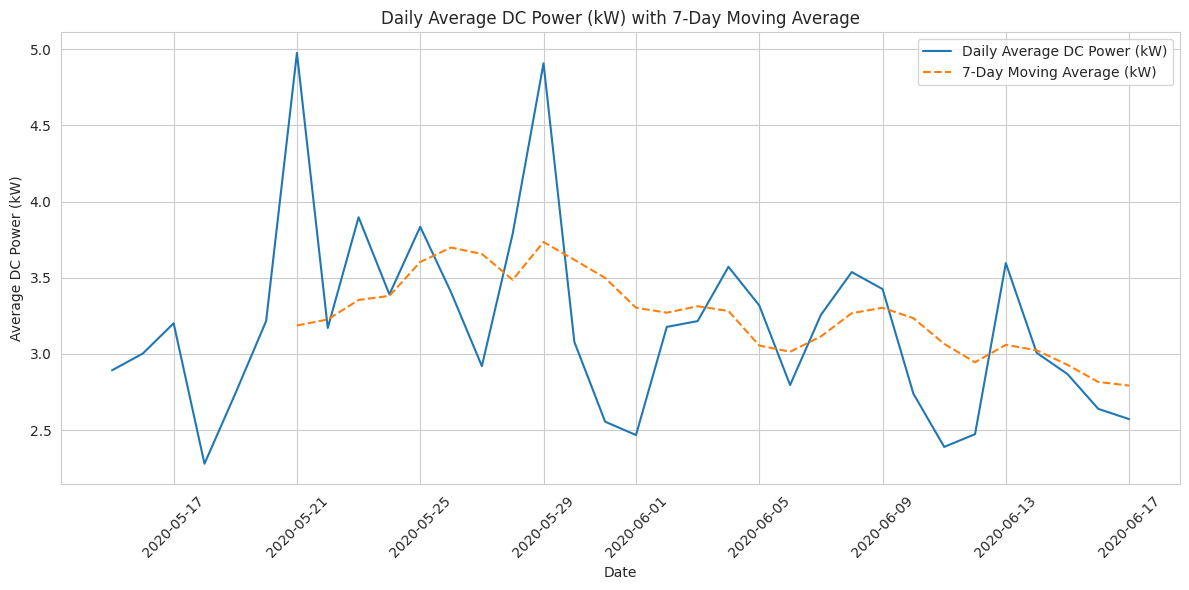
\includegraphics[width=\linewidth]{Figures/dc_by_date_f.png}
    \caption{Average DC Power by Date and 7-Day Moving Average}
    \label{fig:dc_by_date}
\end{figure}

\begin{figure}[!htpb]
    \centering
    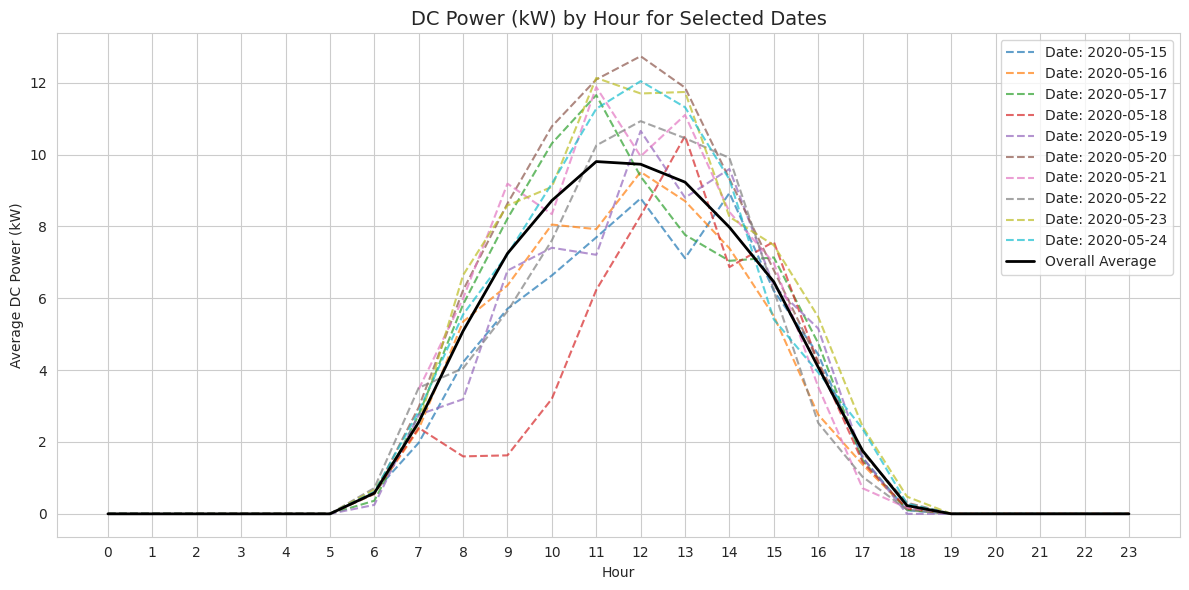
\includegraphics[width=\linewidth]{Figures/dc_by_hour_f.png}
    \caption{DC Power by Hour for a Selection of Dates and Overall Mean of the Entire Data}
    \label{fig:dc_by_hour}
\end{figure}

A brief exploratory analysis of the daily and hourly DC power generation patterns, visualized in Figure \ref{fig:dc_by_date} and Figure \ref{fig:dc_by_hour}, provide insights into the typical power output behavior and the influence of daily and hourly cycles.

\subsection{Data Preprocessing}

Prior to model training and analysis, the raw datasets underwent a series of preprocessing steps:

\begin{enumerate}
   \item \textbf{Data Loading and Resampling:} Both datasets were loaded into the Python environment, with the date-time columns being converted into a consistent and analysis-friendly format. The initial 15-minute frequency of data collection was resampled into two different datasets with both daily and hourly aggregations. This provided flexibility in exploring models sensitive to different temporal resolutions.
   \item \textbf{Merging Datasets:} The generation and weather data were merged into a unified dataset based on their corresponding date-time stamps. This ensured that weather features and power generation values were properly aligned for each observation.
   \item \textbf{Feature Engineering:} Lagged features, representing past values of DC power and weather variables, were generated. These lagged features aimed to capture potential time-dependent patterns and enhance the predictive power of the models.
   \item \textbf{Imputation:} The KNN Imputer was employed to address any remaining missing values in the dataset. This method leverages the values of neighboring data points to estimate and fill in missing entries, preserving data integrity for model training.
\end{enumerate} 

It is important to note that data normalization was skipped, despite it usually being a crucial step in machine learning pipelines, to preserve the original scale of the data and provide a clearer sense of the models' performance metrics.

\subsection{Model}

This study explored both linear and non-linear modeling approaches, with variations in hyperparameter settings, to comprehensively evaluate their effectiveness in predicting DC power generation:

\begin{enumerate}
   \item \textbf{LASSO Regression:} A linear regression technique that incorporates L1 regularization, adding a penalty to model complexity and shrinking coefficients of less important features. This model was implemented with a default regularization parameter.
   \item \textbf{LassoCV (LASSO Regression with Cross-Validation):} Extends LASSO regression by using cross-validation to find the optimal regularization parameter (\(\lambda\)).  LassoCV tested a range of  \(\lambda\) values from 0.001 to 1 to prevent overfitting and select relevant features. Time series cross-validation (TimeSeriesSplit), implementation as seen in Figure \ref{fig:time_series_split} was specifically employed to respect the temporal order of the data during model evaluation.
   \item \textbf{kNN (k-Nearest Neighbors):} A non-parametric method that predicts an output based on the values of its \emph{k} nearest neighbors in the feature space. This model was implemented using hyperparameter tuning for an automated selection of the best \emph{k} neighbors. The model explored \emph{k} values from 3 to 6 to minimize prediction error. 
   \item \textbf{kNN with Cross-Validation:} Improves upon the basic kNN by using cross-validation on top of hyperparameter tuning to determine the optimal number of neighbors (\emph{k}). Similar to LassoCV, time series cross-validation was used to maintain temporal consistency during model assessment. 
\end{enumerate} 

\begin{figure}[!htpb]
    \centering
    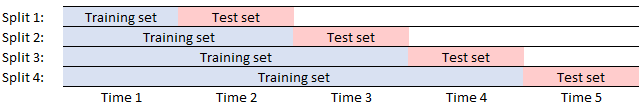
\includegraphics[width=\linewidth]{Figures/time_series_split.png}
    \caption{Expanding Window in scikit-learn's TimeSeriesSplit}
    \label{fig:time_series_split}
\end{figure}

All models were trained using an 80\% split of the data and tested on the remaining 20\%, with a temporally consistent division without shuffling to preserve the continuity of the time series and prevent data leakage.

\subsection{Experiments}

Here, and in the proceeding sections we abbreviate several terms: $D$ for DC power, $A$ for ambient temperature, $M$ for module temperature, and $I$ for irradiation. To evaluate the performance of LASSO and kNN under various scenarios, the following experiments were designed:

\begin{enumerate}

   \item \textbf{Univariate One-day-ahead Prediction with 1 Lag:} This experiment focused on predicting the current day's average DC power solely based on the previous day's average DC power.

\begin{tikzpicture}[
  node distance=.1cm and 1.2cm,
  feature/.style={draw=none},
  target/.style={draw=none}
]

% Matrix with reduced column separation
\matrix (matrix1) [matrix of nodes, column sep=5pt] {
  $\bar{D_0}$ \\ 
  $\bar{D_1}$ \\ 
  \vdots \\
  $\bar{D_{25}}$ \\
  $\bar{D_{26}}$ \\
  $\bar{D_{27}}$  \\
  \vdots \\
  $\bar{D_{32}}$ \\ 
};

% Target column (D) - referencing matrix nodes
\node[target,right=of matrix1-1-1] (D1t) {$\bar{D_1}$};
\node[target,right=of matrix1-2-1] (D2t) {$\bar{D_2}$};
\node[target,below=.001cm of D2t] (dots2) {$\vdots$};
\node[target,right=of matrix1-4-1] (D26t) {$\bar{D_{26}}$};
\node[target,right=of matrix1-5-1] (D27t) {$\bar{D_{27}}$};
\node[target,right=of matrix1-6-1] (D28t) {$\bar{D_{28}}$};
\node[target,below=.001cm of D28t] (dots4) {$\vdots$};
\node[target,right=of matrix1-8-1] (D33t) {$\bar{D_{33}}$};

% Arrows - referencing matrix nodes
\draw[->] (matrix1-1-1) -- node[above,midway,red] {Day 1} (D1t);
\draw[->] (matrix1-2-1) -- node[above,midway,red] {Day 2} (D2t);
\draw[->] (matrix1-4-1) -- node[above,midway,red] {Day 26} (D26t);
\draw[->] (matrix1-5-1) -- node[above,midway,red] {Day 27} (D27t);
\draw[->] (matrix1-6-1) -- node[above,midway,red] {Day 28} (D28t);
\draw[->] (matrix1-8-1) -- node[above,midway,red] {Day 33} (D33t);

\end{tikzpicture}

   \item \textbf{Multivariate (Multiple Features) One-day-ahead Prediction with 1 Lag:} This experiment expanded upon the previous one by incorporating additional lagged features, including daily average ambient temperature, module temperature, and irradiation. The goal was to assess whether the inclusion of these extra features improved predictive accuracy.

\begin{tikzpicture}[
  node distance=.1cm and 1.2cm,
  feature/.style={draw=none},
  target/.style={draw=none}
]

% Matrix with reduced column separation
\matrix (matrix1) [matrix of nodes, column sep=5pt] {
  $\bar{D_0}$ & $\bar{I_0}$ & $\bar{A_0}$ & $\bar{M_0}$ \\ 
  $\bar{D_1}$ & $\bar{I_1}$ & $\bar{A_1}$ & $\bar{M_1}$ \\ 
  \vdots & \vdots & \vdots & \vdots \\
  $\bar{D_{25}}$ & $\bar{I_{25}}$ & $\bar{A_{25}}$ & $\bar{M_{25}}$ \\
  $\bar{D_{26}}$ & $\bar{I_{26}}$ & $\bar{A_{26}}$ & $\bar{M_{26}}$ \\
  $\bar{D_{27}}$ & $\bar{I_{27}}$ & $\bar{A_{27}}$ & $\bar{M_{27}}$ \\
  \vdots & \vdots & \vdots & \vdots \\
  $\bar{D_{32}}$ & $\bar{I_{32}}$ & $\bar{A_{32}}$ & $\bar{M_{32}}$ \\ 
};

% Target column (D) - referencing matrix nodes
\node[target,right=of matrix1-1-4] (D1t) {$\bar{D_1}$};
\node[target,right=of matrix1-2-4] (D2t) {$\bar{D_2}$};
\node[target,below=.001cm of D2t] (dots2) {$\vdots$};
\node[target,right=of matrix1-4-4] (D26t) {$\bar{D_{26}}$};
\node[target,right=of matrix1-5-4] (D27t) {$\bar{D_{27}}$};
\node[target,right=of matrix1-6-4] (D28t) {$\bar{D_{28}}$};
\node[target,below=.001cm of D28t] (dots4) {$\vdots$};
\node[target,right=of matrix1-8-4] (D33t) {$\bar{D_{33}}$};

% Arrows - referencing matrix nodes
\draw[->] (matrix1-1-4) -- node[above,midway,red] {Day 1} (D1t);
\draw[->] (matrix1-2-4) -- node[above,midway,red] {Day 2} (D2t);
\draw[->] (matrix1-4-4) -- node[above,midway,red] {Day 26} (D26t);
\draw[->] (matrix1-5-4) -- node[above,midway,red] {Day 27} (D27t);
\draw[->] (matrix1-6-4) -- node[above,midway,red] {Day 28} (D28t);
\draw[->] (matrix1-8-4) -- node[above,midway,red] {Day 33} (D33t);

\end{tikzpicture}

   \item \textbf{Multivariate (Hourly Train Data as Features) One-day-ahead Prediction with 1 Lag:} Recognizing the potential value of higher temporal granularity, this experiment used the previous day hourly weather data and lagged features to predict current day average DC power. Various combinations of features were explored through feature selection.

\begin{tikzpicture}[
  node distance=.1cm and 1.2cm,
  feature/.style={draw=none},
  target/.style={draw=none}
]

% Matrix with reduced column separation and repeated elements
\matrix (matrix1) [matrix of nodes, column sep=5pt, nodes={align=center}] {
  $D^1_0$ & \dots & $D^{24}_0$  & \dots & $I^1_0$ & \dots & $I^{24}_0$ \\[-3pt]
  $D^1_1$ & \dots & $D^{24}_1$  & \dots & $I^1_1$ & \dots & $I^{24}_1$ \\[-3pt] 
  \vdots &  & \vdots & & \vdots &  & \vdots \\
  $D^1_{25}$ & \dots & $D^{24}_{25}$  & \dots & $I^1_{25}$ & \dots & $I^{24}_{25}$ \\[-3pt] 
  $D^1_{26}$ & \dots & $D^{24}_{26}$  & \dots & $I^1_{26}$ & \dots & $I^{24}_{26}$ \\[-3pt]
  $D^1_{27}$ & \dots & $D^{24}_{27}$  & \dots & $I^1_{27}$ & \dots & $I^{24}_{27}$ \\[-3pt]
  \vdots &  & \vdots & & \vdots &  & \vdots \\
  $D^1_{32}$ & \dots & $D^{24}_{32}$  & \dots & $I^1_{32}$ & \dots & $I^{24}_{32}$ \\ 
};

% Target column (D) - referencing matrix nodes
\node[target,right=of matrix1-1-7] (D1t) {$\bar{D_1}$};
\node[target,right=of matrix1-2-7] (D2t) {$\bar{D_2}$};
\node[target,below=-0.1cm of D2t] (dots2) {$\vdots$};
\node[target,right=of matrix1-4-7] (D26t) {$\bar{D_{26}}$};
\node[target,right=of matrix1-5-7] (D27t) {$\bar{D_{27}}$};
\node[target,right=of matrix1-6-7] (D28t) {$\bar{D_{28}}$};
\node[target,below=-0.1cm of D28t] (dots4) {$\vdots$};
\node[target,right=of matrix1-8-7] (D33t) {$\bar{D_{33}}$};

% Arrows - referencing matrix nodes
\draw[->] (matrix1-1-7) -- node[above,midway,red] {Day 1} (D1t);
\draw[->] (matrix1-2-7) -- node[above,midway,red] {Day 2} (D2t);
\draw[->] (matrix1-4-7) -- node[above,midway,red] {Day 26} (D26t);
\draw[->] (matrix1-5-7) -- node[above,midway,red] {Day 27} (D27t);
\draw[->] (matrix1-6-7) -- node[above,midway,red] {Day 28} (D28t);
\draw[->] (matrix1-8-7) -- node[above,midway,red] {Day 33} (D33t);

\end{tikzpicture}

\end{enumerate} 

\subsection{Evaluation}

Model performance was rigorously evaluated using the Root Mean Squared Error (RMSE) metric. RMSE quantifies the average magnitude of prediction errors, providing a measure of how well the model's predictions align with the actual DC power values. Lower RMSE values indicate better predictive accuracy.

$RMSE: \sqrt{\frac{1}{6}\sum_{i=1}^{6} \left[ (y_{test})_i - Model.Predict(x_{test})_i \right]^2}$

A comparative analysis of RMSE scores across all experiments helped determine the most effective modeling approach for this specific problem. The analysis considered factors such as feature set selection, temporal resolution of the data, and the influence of hyperparameter tuning on each model's predictive accuracy.
\section{Results and Discussion}

This section discusses the findings of the experiments, analyzing the strengths and weaknesses of the proposed models. The analysis focuses on the following aspects:

\begin{itemize}
    \item \textbf{Effectiveness and comparison of the models:} Each model's performance at different frequencies and the reasons for their effectiveness.
    
    \item \textbf{Limitations of the approach:} Potential limitations of each model.
    
    \item \textbf{Future work:} Future directions that could be explored to improve the performance of the models.
\end{itemize}

\subsection{Effectiveness and Comparison of the Models}

Initially, we focused on predicting daily average DC power using both univariate (only lagged DC power) and multivariate (including lagged ambient temperature, module temperature, and irradiation) setups.

\begin{figure}[h]
    \centering
    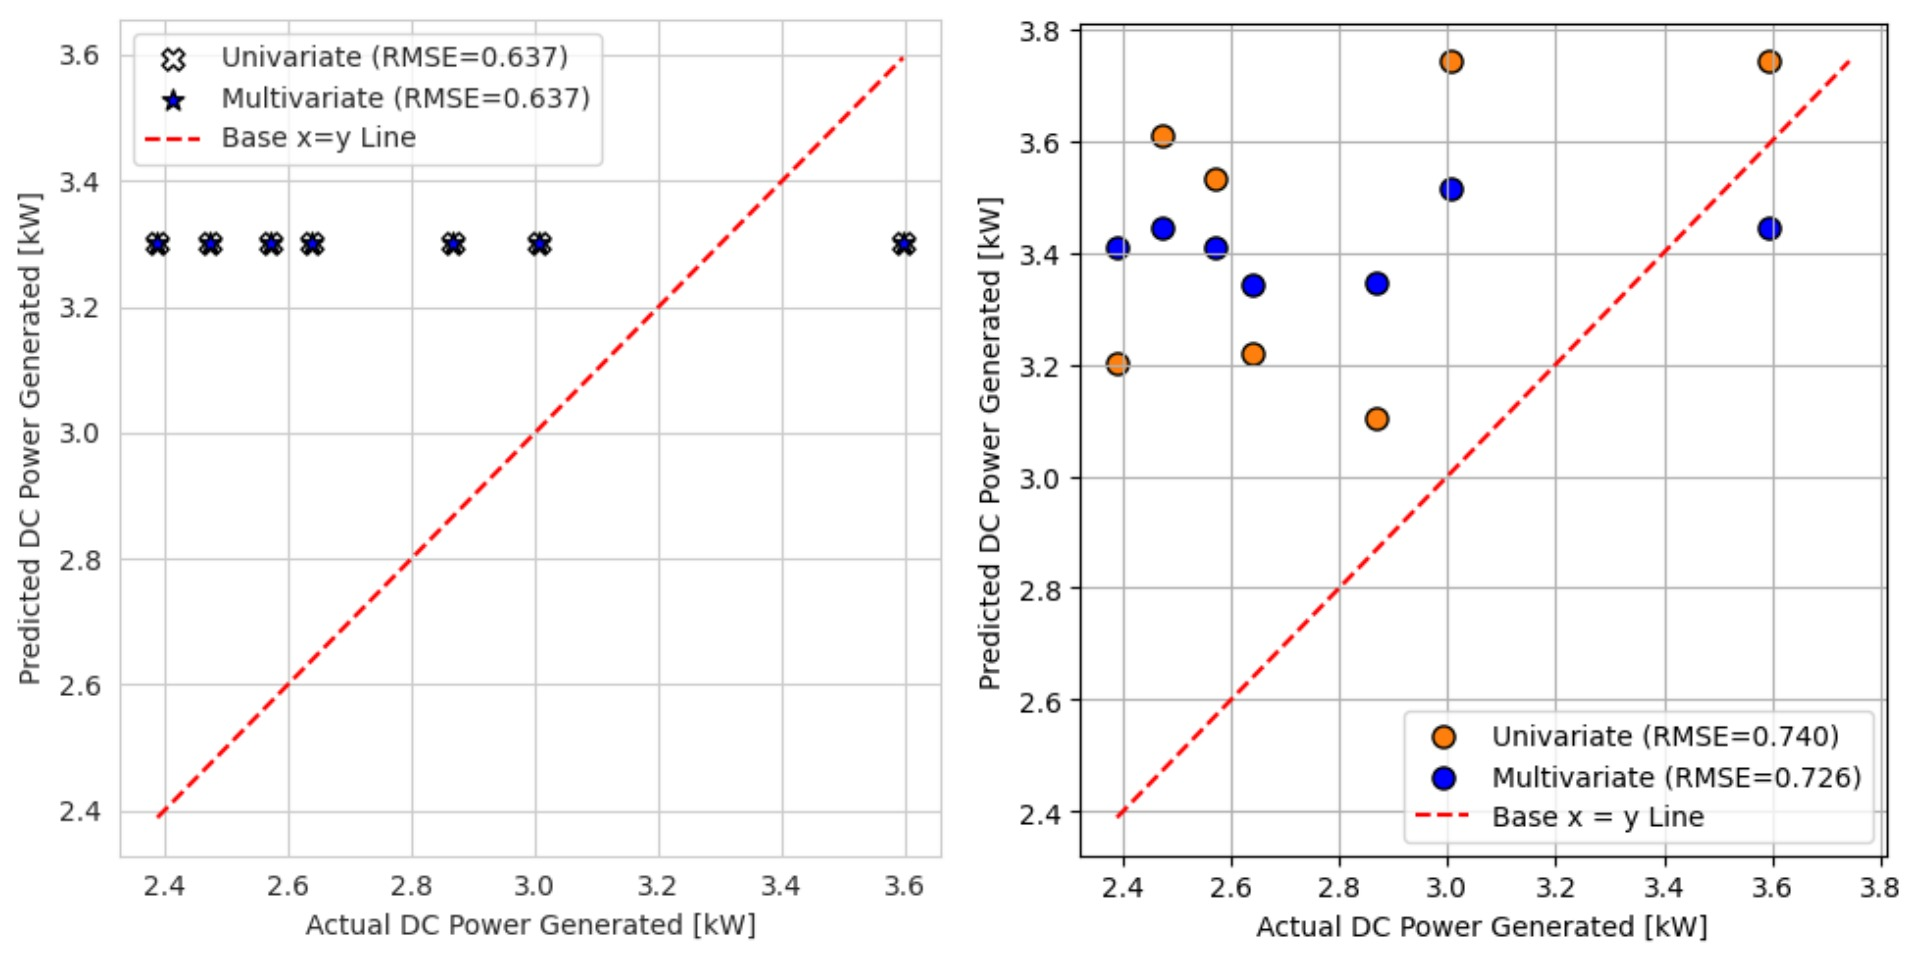
\includegraphics[width=0.5\textwidth]{Figures/uni-multi.jpg}
    \caption{Univariate with only DC Power and Multivariate: Actual vs Predicted for LASSO (left) and kNN (right)}
    \label{fig:uni-multi}
\end{figure}

As shown in Figure \ref{fig:uni-multi}, for the daily prediction frequency, the LASSO model with feature sets ($D$) and ($D$, $A$, $I$, $M$) both achieved an RMSE of 0.637. The kNN model performed slightly worse, with RMSE values of 0.740 for feature set ($D$) and 0.726 for feature set ($D$, $A$, $I$, $M$). This indicates that for daily predictions, the LASSO model is more effective. It's important to note that in both univariate and multivariate settings, the LASSO model, which utilized the default alpha (\(\lambda\)) value of 1.0, exhibited a particular behavior. When alpha is set to 1.0, the regularization penalty is high, leading to the coefficient for DC power being shrunk to zero for the univariate model and all the other features including DC power in the multivariate model. This effectively nullifies the influence of these features on the prediction. In such a scenario, the LASSO model relies solely on the intercept term to make predictions. Consequently, regardless of the input, the model will always predict the average DC power observed during training.
This behavior explains the consistent RMSE value of 0.637 for LASSO in both the univariate and multivariate daily predictions. While LASSO technically outperforms kNN in these cases, its predictive power is limited by the high regularization strength, rendering it equivalent to a simple average predictor. However, the high RMSE values for both models highlight the lack of precision we encountered. Therefore, we transitioned to hourly training data to aim for an RMSE of 0.5 or lower, and perform hyperparamter tuning to achieve better regularization.

On an hourly basis, we examined which features were most relevant and how well each algorithm could capture the trend. It was found that Irradiation and DC power were the most informative features, likely due to their high correlation, as depicted in Figure \ref{fig:hourDC}.

\begin{figure}[h]
    \centering
    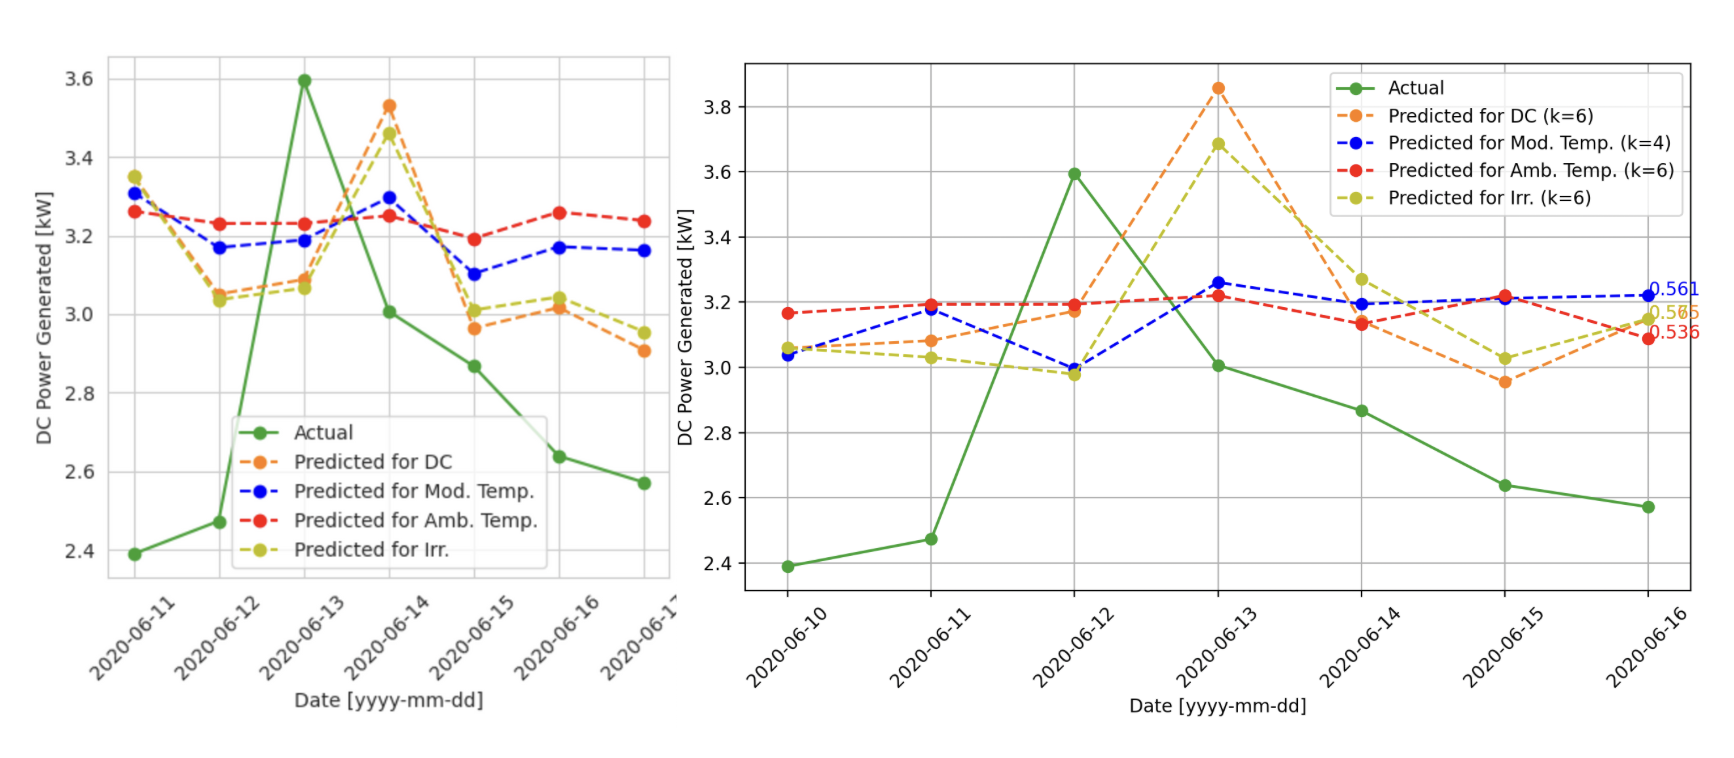
\includegraphics[width=0.5\textwidth]{Figures/hourDC.png}
    \caption{Trends for univariate prediction with time series cross-validation on an hourly training basis: LASSO (left) and kNN (right)}
    \label{fig:hourDC}
\end{figure}

However, even with time series cross-validation and hyperparameter tuning in multivariate settings with DC power as a reference feature, we were unable to improve the models' ability to capture the intra-day variations in DC power. This is illustrated in Figure \ref{fig:hourDCF}.

\begin{figure}[h]
    \centering
    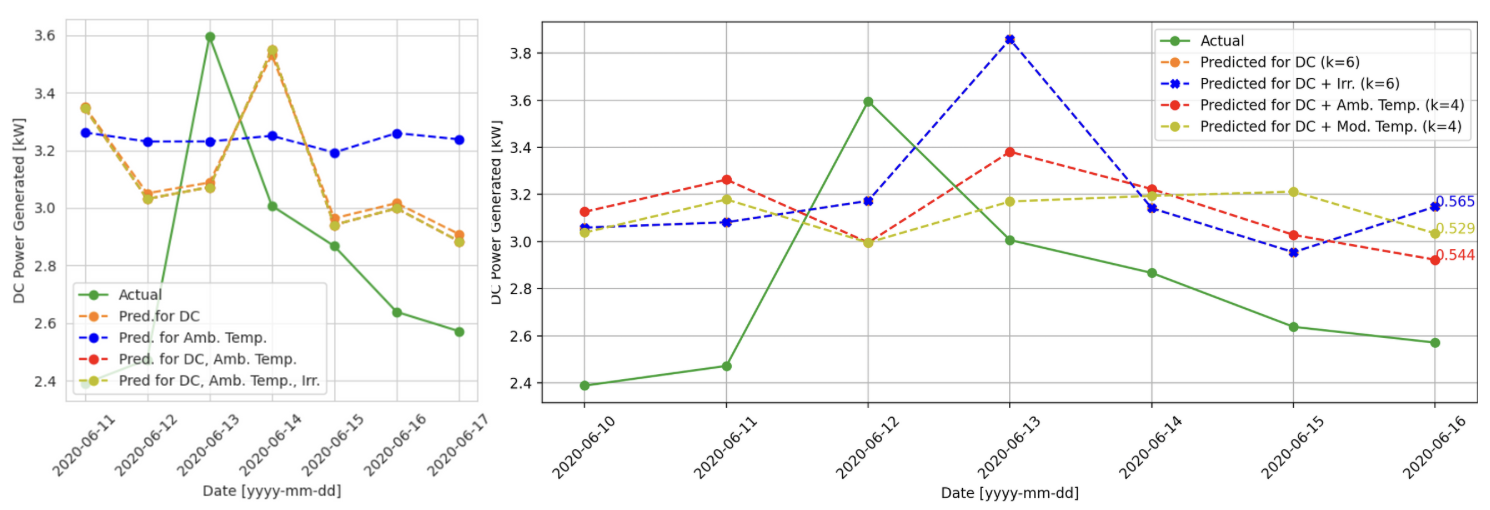
\includegraphics[width=0.5\textwidth]{Figures/hourDCF.png}
    \caption{Trends for multivariate with feature set combinations: LASSO (left) and kNN (right)}
    \label{fig:hourDCF}
\end{figure}

\begin{figure}[h]
    \centering
    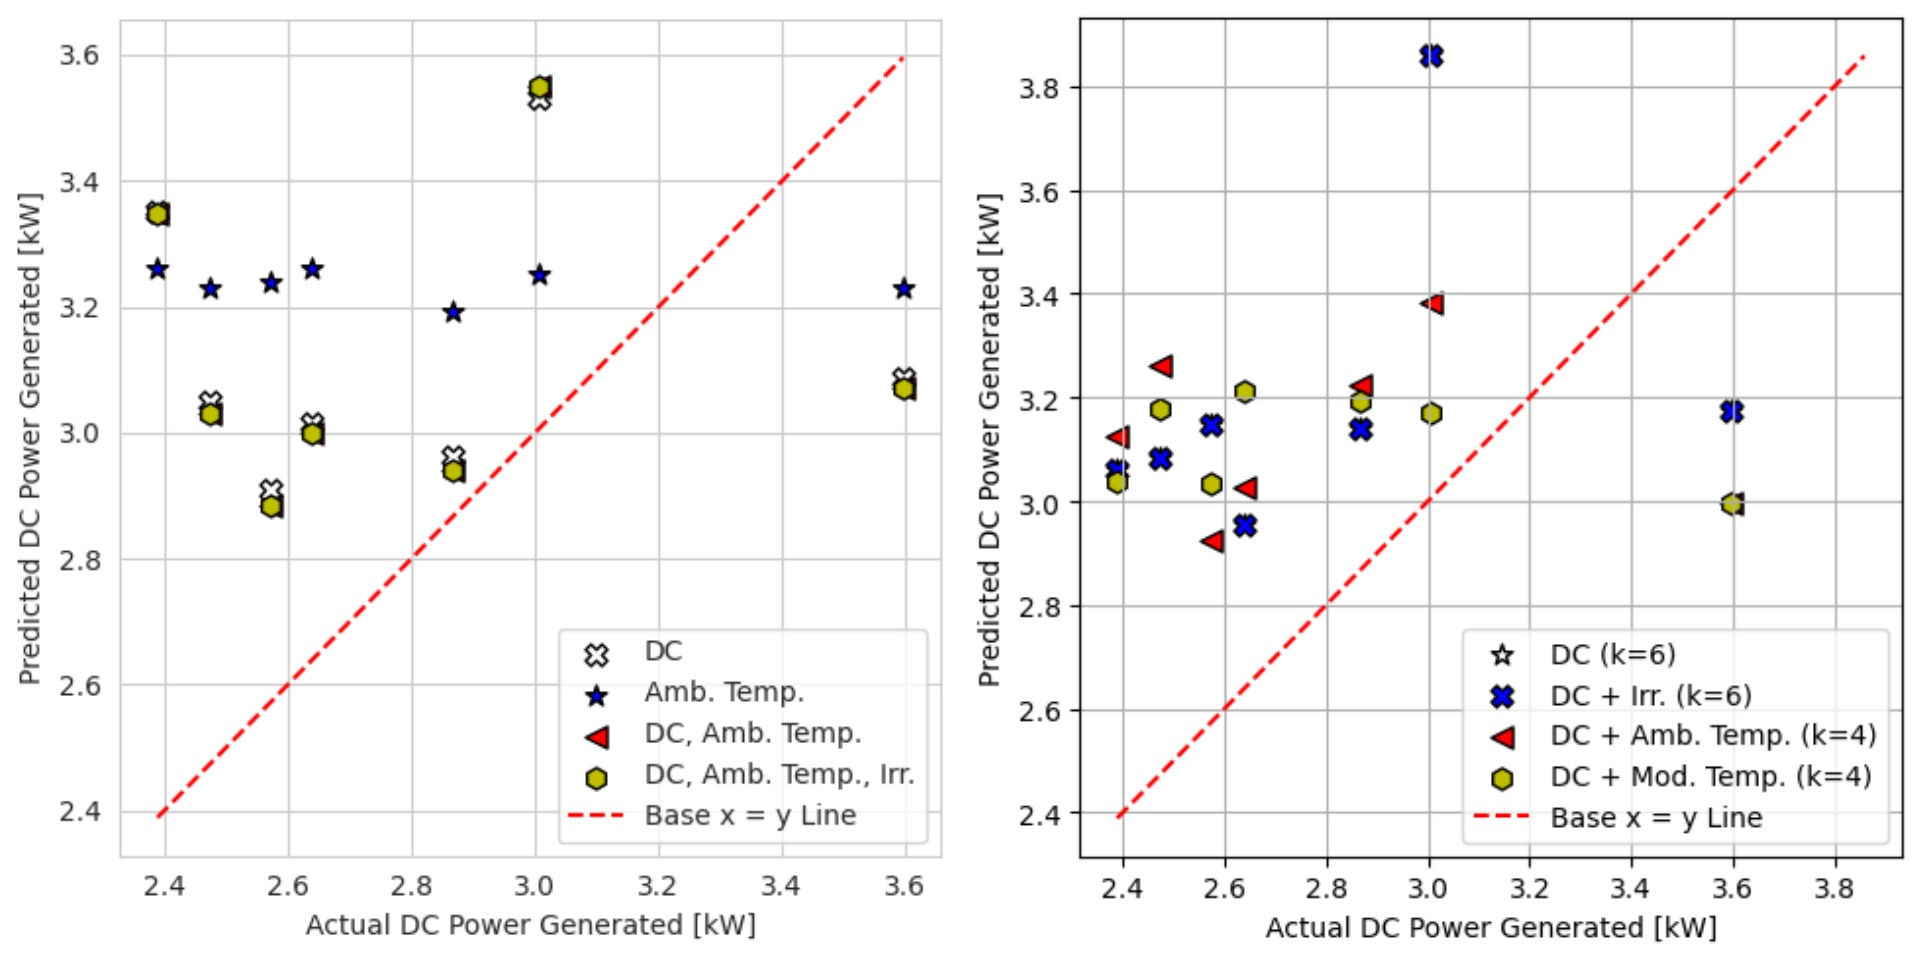
\includegraphics[width=0.5\textwidth]{Figures/multi_pred_vs_actual.jpg}
    \caption{Multivariate with feature set combinations: Actual vs Predicted for LASSO (left) and kNN (right)}
    \label{fig:multi-pred-actual}
\end{figure}

As shown in Figure \ref{fig:multi-pred-actual}, both models tend to overpredict on average, which suggests a potential area for future improvement.

\begin{table}[h]
    \centering
    \caption{LASSO coefficient selection with feature combinations}
    \begin{tabular}{|l|l|l|l|l|l|l|} 
    \hline
    $\beta_h$ & $h=1$ & $h=2$ & $h=3$ & $h=4$ & $h=5$ & $h=6$ \\ 
    \hline
    $D$ & 0 & 0 & 0 & 0 & 0 & 0 \\ 
    \hline
    $A$ & 0 & 0 & 0 & 0 & 0 & 0 \\ 
    \hline
    $D,A$ & 0,0 & 0,0 & 0,0 & 0,0 & 0,0 & 0,0 \\ 
    \hline
    $D,A,I$ & 0,0,0 & 0,0,0 & 0,0,0 & 0,0,0 & 0,0,0 & 0,0,0 \\ 
    \hline
    $\beta_h$ & $h=7$ & $h=8$ & $h=9$ & $h=10$ & $h=11$ & $h=12$ \\ 
    \hline
    $D$ & 0 & 0 & 0 & 0 & 0 & \textbf{0.04} \\ 
    \hline
    $A$ & 0 & 0 & 0 & 0 & 0 & 0 \\ 
    \hline
    $D,A$ & 0,0 & 0,0 & 0,0 & 0,0 & 0,0 & \textbf{0.04},0 \\ 
    \hline
    $D,A,I$ & 0,0,0 & 0,0,0 & 0,0,0 & 0,0,0 & 0,0,0 & \textbf{0.04},0,0 \\ 
    \hline
    $\beta_h$ & $h=13$ & $h=14$ & $h=15$ & $h=16$ & $h=17$ & $h=18$ \\ 
    \hline
    $D$ & \textbf{0.08} & 0 & 0 & 0 & 0 & 0 \\ 
    \hline
    $A$ & \textbf{0.01} & 0 & 0 & 0 & 0 & 0 \\ 
    \hline
    $D,A$ & \textbf{0.08},0 & 0,0 & 0,0 & 0,0 & 0,0 & 0,0 \\ 
    \hline
    $D,A,I$ & \textbf{0.08},0,0 & 0,0,0 & 0,0,0 & 0,0,0 & 0,0,0 & 0,0,0 \\ 
    \hline
    $\beta_h$ & $h=19$ & $h=20$ & $h=21$ & $h=22$ & $h=23$ & $h=24$ \\ 
    \hline
    $D$ & 0 & 0 & 0 & 0 & 0 & 0 \\ 
    \hline
    $A$ & \textbf{0.02} & 0 & 0 & 0 & 0 & 0 \\ 
    \hline
    $D,A$ & 0,0 & 0,0 & 0,0 & 0,0 & 0,0 & 0,0 \\ 
    \hline
    $D,A,I$ & 0,0,0 & 0,0,0 & 0,0,0 & 0,0,0 & 0,0,0 & 0,0,0 \\ 
    \hline
    \end{tabular}
    \label{tab:coeff_lasso}
\end{table}

A detailed examination of the LASSO coefficient table (Table \ref{tab:coeff_lasso}) indicates that most coefficients, even during peak power generation hours (6 AM to 6 PM), are zero. This sparsity highlights LASSO's tendency to select only the most critical features, effectively ignoring others. Notably, specific hours such as hour 12 and 13 are used by LASSO, reinforcing the model's focus on particular time slots for prediction. Furthermore, analysis of the alpha vs. RMSE graph (Figure \ref{fig:rmse-vs-alpha}) demonstrates that adding more than two feature combinations results in similar outcomes, effectively removing those additional features from being used in training. This behavior underscores the importance of feature selection in optimizing model performance without overfitting.

\subsection{Limitations of the Approach}

The primary limitation we encountered stemmed from the dataset itself. The high volatility inherent in daily power output, combined with the relatively small sample size (34 days), likely hindered the models' ability to discern clear patterns.

This issue also affected the cross-validation step, as the small number of points in the test set (only 7) restricted the applicability of kNN for a higher number of neighbors, as shown in Figure \ref{fig:CV_F_Evo}.

\begin{figure}[h]
    \centering
    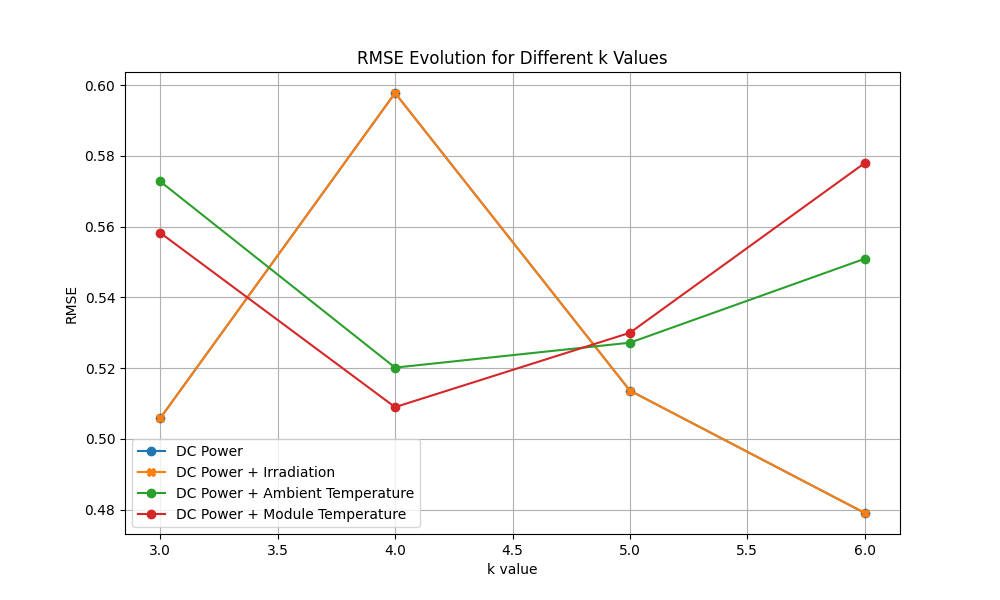
\includegraphics[width=0.5\textwidth]{Figures/CV_F_Evo.png}
    \caption{Evolution of RMSE as a function of the number of neighbors $k$ in the kNN algorithm for multivariate with feature set combinations}
    \label{fig:CV_F_Evo}
\end{figure}

Increasing the test set size to ten points confirmed this theory, allowing kNN to achieve an RMSE of 0.49 using DC power and module temperature as combined features.

It may be noticed that LASSO algorithm seemed to not be sensitive to this issue.

\begin{figure}[h]
    \centering
    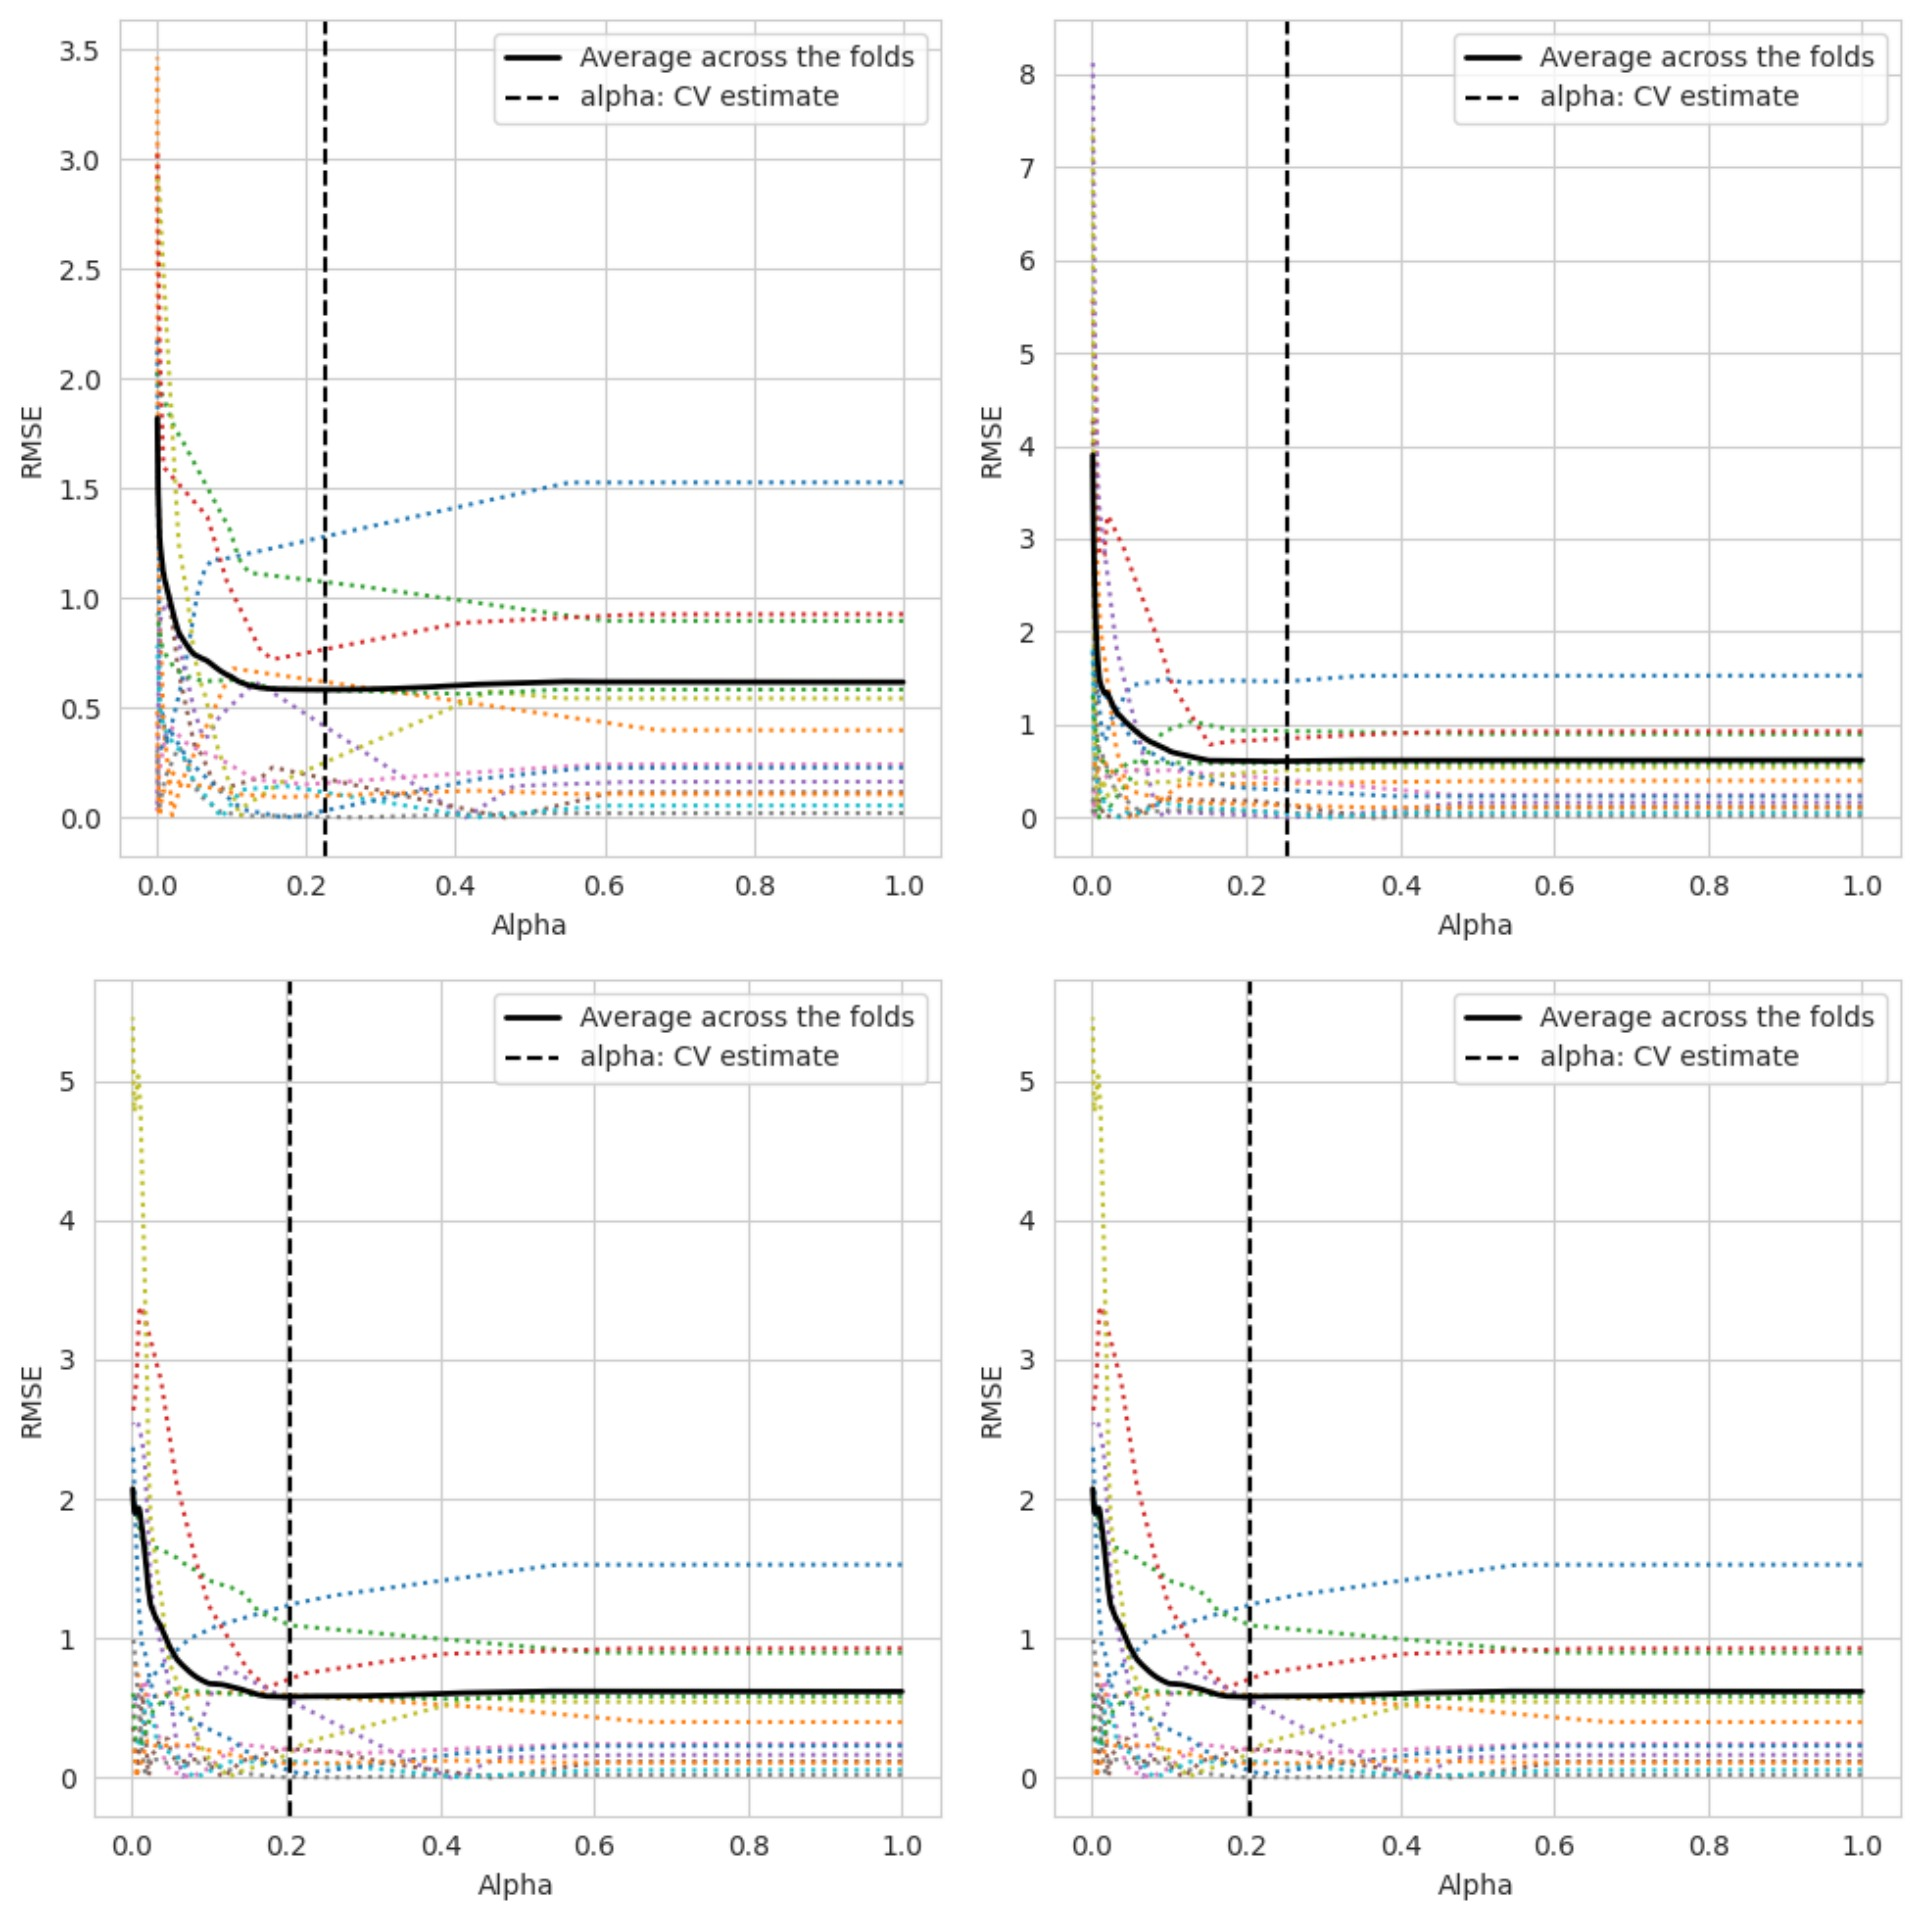
\includegraphics[width=0.5\textwidth]{Figures/rmse_vs_alpha_lasso.jpg}
    \caption{RMSE vs. regularization strength ($\lambda$) for LASSO models with varying feature sets. (Top left) DC power only, (top right) Ambient temperature only, (bottom left) DC power and ambient temperature, and (bottom right) DC power, ambient temperature, and irradiation}
    \label{fig:rmse-vs-alpha}
\end{figure}

\subsection{Future Work}

Future research could explore the following directions:

\begin{itemize}
    \item \textbf{Data processing:} Increase the dataset length or use a different dataset with more samples to improve the models' ability to capture trends and reduce the impact of volatility. A larger and more diverse dataset could enhance the robustness of the predictions.
    \item \textbf{Advanced Modeling Techniques:} Explore and implement advanced machine learning algorithms such as Random Forest, Gradient Boosting Machines, or Deep Learning models. These methods may provide better performance by capturing complex patterns in the data.
    \item \textbf{Feature Engineering:} Investigate additional features that could improve prediction accuracy, such as incorporating weather forecasts, historical power generation data, and real-time sensor data.
    \item \textbf{Optimization Techniques:} Further fine-tune hyperparameters using advanced optimization methods like Bayesian Optimization.
\end{itemize}

\begin{table}[h]
    \centering
    \caption{Model Performance for Predicting Current Day Average DC Power}
    \begin{tabular}{|l|l|l|r|r|r|} 
    \hline
    \textbf{Model} & \textbf{Frequency} & \textbf{Features} & \textbf{$k$} & \textbf{$\lambda$} & \textbf{RMSE} \\ \hline
    Lasso & Day & $D$ & - & 1.0 & 0.637 \\ \hline
    Lasso & Day & $D$, $A$, $I$, $M$ & - & 1.0 & 0.637 \\ \hline
    LassoCV & Hour & $D$ & - & 0.225 & 0.542 \\ \hline
    LassoCV & Hour & $A$ & - & 0.253 & 0.593 \\ \hline
    \textbf{LassoCV} & \textbf{Hour} & \textbf{$D$, $A$} & - & \textbf{0.206} & \textbf{0.538} \\ \hline
    LassoCV & Hour & $D$, $A$, $I$ & - & 0.206 & 0.538 \\ \hline
    kNN & Day & $D$ & 7 & - & 0.740 \\ \hline
    kNN & Day & $D$, $A$, $I$, $M$ & 7 & - & 0.726 \\ \hline
    kNN CV & Hour & $D$ & 6 & - & 0.565 \\ \hline
    kNN CV & Hour & $A$ & 6 & - & 0.536 \\ \hline
    kNN CV & Hour & $I$ & 4 & - & 0.570 \\ \hline
    kNN CV & Hour & $M$ & 6 & - & 0.561 \\ \hline
    kNN CV & Hour & $D$ & 6 & - & 0.565 \\ \hline
    kNN CV & Hour & $D$, $A$ & 4 & - & 0.544 \\ \hline
    \textbf{kNN CV} & \textbf{Hour} & \textbf{$D$, $M$} & \textbf{4} & - & \textbf{0.529} \\ \hline
    \end{tabular}
    \label{tab:model_comparison}
\end{table}
% Conclusion
\section{Conclusion}
Based on the comparative analysis of machine learning models for predicting solar power generation from weather conditions and lagged features, several insights have emerged:

The study evaluated Lasso regression and kNN regression across different scenarios, including univariate and multivariate setups with daily and hourly data. Results indicated that Lasso regression generally outperformed kNN in both daily predictions and hourly predictions, even if kNN hit the lowest RMSE while sacrificing the trend catch. However, both models struggled to achieve desired accuracy levels, particularly in hourly predictions where the RMSE hovered around 0.5 or higher. The best performing models (Table \ref{tab:model_comparison}) were LassoCV (RMSE of 0.538 using lagged DC power and ambient temperature) and kNN with cross-validation (RMSE of 0.529 using lagged DC power and module temperature).

Challenges such as dataset volatility and limited sample size impacted model performance, particularly in capturing finer temporal trends. Despite efforts in feature engineering and model tuning, including cross-validation and hyperparameter optimization, achieving precise predictions remained elusive.

In conclusion, while Lasso regression showed promise in daily predictions, enhancing data quality and model sophistication is necessary to improve forecasting accuracy for solar power generation. These improvements would also benefit kNN, as highlighted earlier. Future research should focus on acquiring a larger dataset, engineering domain-specific features, and exploring advanced time series models to address these challenges and further refine predictive capabilities in renewable energy forecasting.

\section*{Acknowledgements}
This research received support during the ResProj course, from Professor Motonobu KANAGAWA and Ms. Parastoo PASHMCHI.

\begin{thebibliography}{9}

\bibitem{arxiv1802.03913}
Assessing the Utility of Weather Data for Photovoltaic Power Prediction (2018).
\url{https://arxiv.org/abs/1802.03913}

\bibitem{arxiv1710.03803}  
Day-Ahead Solar Forecasting Based on Multi-level Solar Measurements (2017).
\url{https://arxiv.org/abs/1710.03803}

\bibitem{arxiv2403.01653}
Day-ahead regional solar power forecasting with hierarchical temporal convolutional neural networks using historical power generation and weather data (2024). 
\url{https://arxiv.org/abs/2403.01653}

\bibitem{arxiv2109.13442}
An Adaptive Deep Learning Framework for Day-ahead Forecasting of Photovoltaic Power Generation (2021).
\url{https://arxiv.org/abs/2109.13442}

\bibitem{arxiv2011.09950}
Improving Solar and PV Power Prediction with Ensemble Methods (2020).
\url{https://arxiv.org/abs/2011.09950}

\bibitem{ieee8306874}
Solar Power Generation Forecasting With a LASSO-Based Approach (2018).
\url{https://ieeexplore.ieee.org/document/8306874}

\bibitem{ieee8066360}
Day-Ahead Hourly Forecasting of Power Generation From Photovoltaic Plants (2017).
\url{https://ieeexplore.ieee.org/document/8066360}

\bibitem{arxiv2104.07352}
Day-Ahead and Intra-Day Planning of Integrated BESS-PV Systems providing Frequency Regulation (2021).
\url{https://arxiv.org/abs/2104.07352}

\bibitem{arxiv2301.05911}
Day-Ahead PV Power Forecasting Based on MSTL-TFT (2023).
\url{https://arxiv.org/abs/2301.05911}

\bibitem{atlantis125995001}
Trend-Based K-Nearest Neighbor Algorithm in Stock Price Prediction (2023).
\url{https://www.atlantis-press.com/proceedings/deca-23/125995001}

\bibitem{solar-kaggle}
Pietro Michiardi. Solar Power Generation Data – Solar power generation and sensor data for two power plants.
\url{https://www.kaggle.com/datasets/anikannal/solar-power-generation-data}.
2020.

\end{thebibliography}

\end{document}